\chapter{Demodulation Challenges}
While analyzing different demodulation algorithms and trying to improve their performance, there were a few phenomena that were observed that made correct demodulation more challenging. The following items created difficulty and can all be attributed to the fact that APRS uses RF and hence is susceptible to all the items relating to an RF transmission. 

The main challenge in decoding the APRS data was the fact that the digital stream is converted to an audio signal and then transmitted over RF. The addition of RF adds a whole plethora of obstacles which can include Path Loss, Multi-path, Fading, Doppler effects, Co-channel interference, Interference and Noise, and Foliage\,\cite{Goleniewski2006}. A few items which are important to note, due to the fact that some of the algorithms had to be coded to tolerate them are: DC Offset, Noise, and Emphasis.

\section{Challenge: DC Offset}
An audio signal can be characterized by a sine wave. In order to get different sounds the frequency of the sine wave is changed and in the context here, the two frequencies are 1200Hz and 2200Hz. Since an audio signal is a sine wave, the average value should be zero. The zero value is commonly referred to as the ground of the audio signal, and as the definition would imply the signal should spend the same amount of time above ground as it does below ground. As the performance of zero crossing algorithms were investigated it was evident that this was a challenge. If one assumes that the signal is centered about zero, and it is not, the logical decisions made with this incorrect assumption will hence not hold true. Figure \ref{DCOffsetExample} shows that the signal is not centered around zero. This lack of the signal being centered around 0 (or ground) is why it is said to have a DC offset. It can be noticed in this figure that near the center there are time periods that would be both much longer and much shorter than those expected from subsequent zero crossings during demodulation due to this DC offset effect.
\begin{figure}
  \centering
	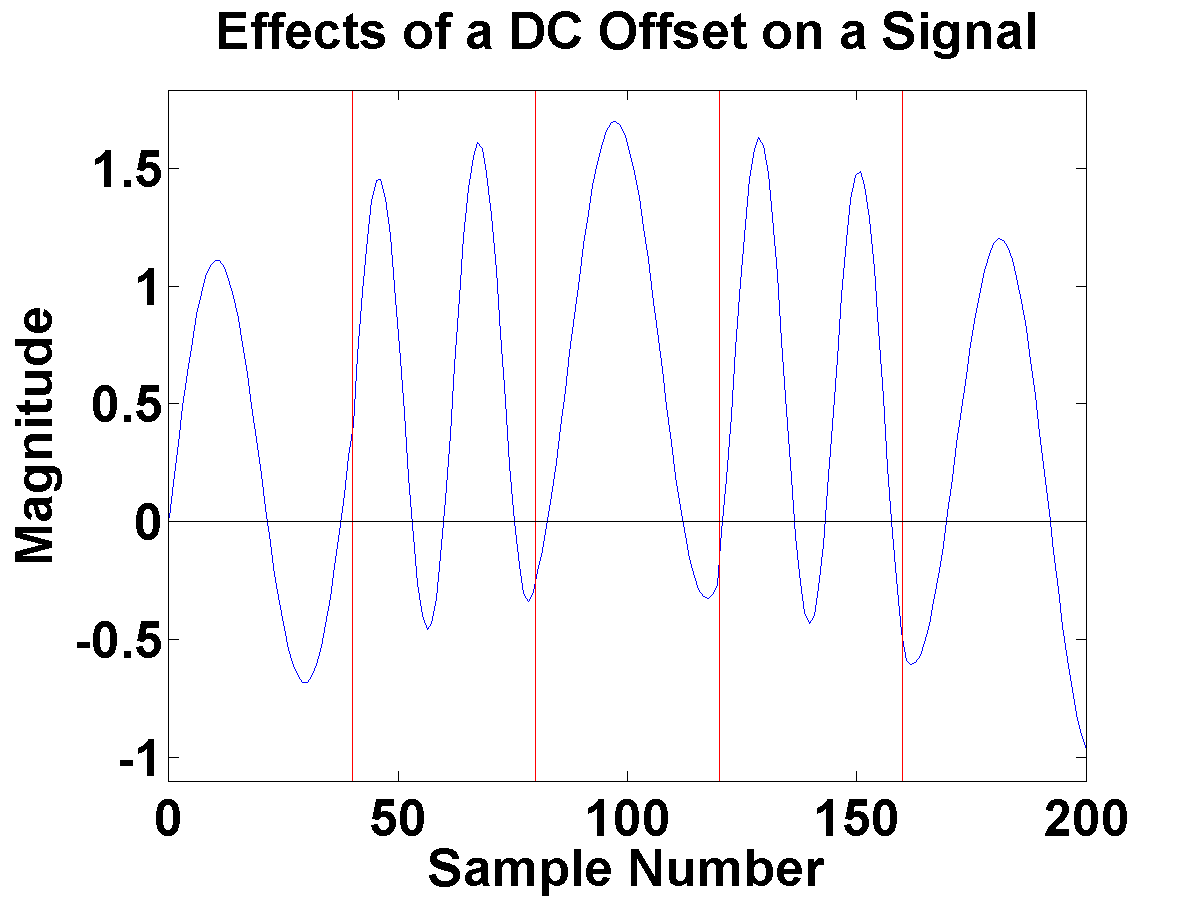
\includegraphics[width=0.75\linewidth]{images/EffectsofaDCOffsetonaSignal.png} 
	\caption{An example Bell 202 signal with DC offset problems.}
   \label{DCOffsetExample}
\end{figure}

\section{Challenge: Noise}
First, a definition of noise in the context of this research: noise refers to unwanted electrical signals present in electrical systems\,\cite{Sklar1988}. Since the data is an AFSK signal that is then frequency modulated, there are two distinct steps where noise can be introduced, but must be kept to a minimum to increase the chances of the data being properly transferred. Hence, a large signal to noise ratio (SNR) is preferred. This is not the case for only APRS but with all wireless technologies. One cause of having an increased effect from noise and hence a lower SNR is increased distance between the transmitter and receiver. An example that many are probably familiar with is as a client gets farther away from a wireless access point the bandwidth decreases. This happens because the signal strength drops off at 1 / distance cubed\,\cite{4Gon}. What was noticed when some of the algorithms were being debugged was the random noise embedded in the signal caused significant problems.

One such example of this is if the noise happened to also take on the form of a sine wave and the algorithm locked onto that frequency instead of the 1200Hz or 2200Hz signal that was wanted to be decoded. Alternatively, if the noise was just random and jostled the signal in the correct spot 1200Hz tones might look like 2200Hz (this ended up being fairly common) or vice versa. An example of what noise may look like on the original signal can be seen in Figure \ref{noiseExample}.
\begin{figure}
  \centering
	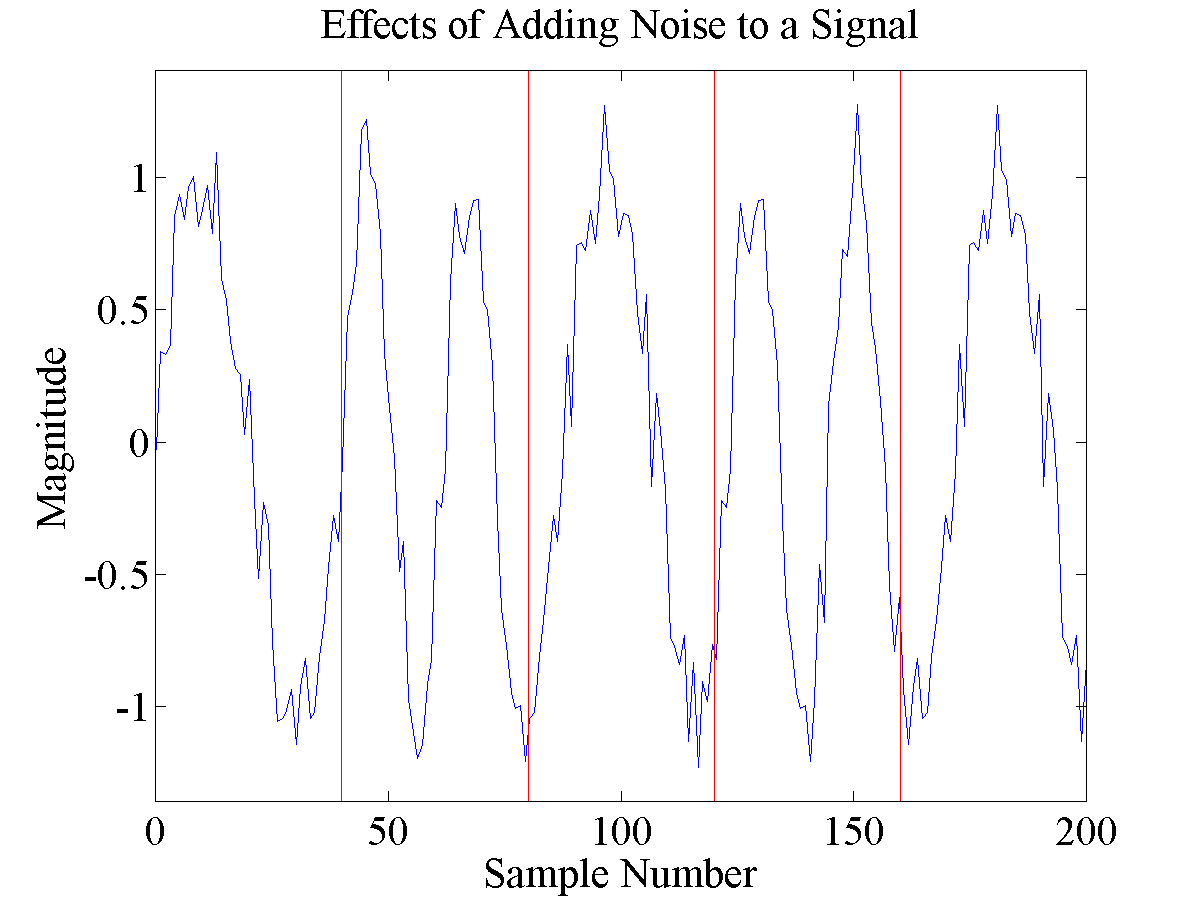
\includegraphics[width=0.75\linewidth]{images/EffectsofAddingNoisetoaSignal.png} 
	\caption[An example Bell 202 signal with white noise added.]{An example Bell 202 signal with white noise added. The additional zero crossings at sample 9 in the first bit period and sample 169 in the last bit period will make these 1200Hz bit periods look more like 2200Hz signals.}
   \label{noiseExample}
\end{figure}

\section{Challenge: Emphasis}
Due to the fact that this is AFSK data being transmitted over a voice channel, emphasis becomes a concern. Preemphasis is when the the higher audio tones in a Frequency Modulated (FM) signal are intentionally increased and deemphasis is when that process is reversed on the receiving end to return the audio to a flat level. Why emphasize the audio signal? This process of emphasis is not necessary, but the effects are desirable since it increases the signal to noise ratio in the RF signal by having the higher audio tones preemphasized\,\cite{Gibilisco1994}. The reason this is a concern is because the adoption of emphasizing and deemphasizing APRS signals is inconsistent. Some radios have data ports which bypass the emphasis step while other APRS users utilize the microphone and speaker ports of a radio which would utilize emphasis. This would mean that a signal transmitted out of a radio with a data port may not be emphasized, but then when received through the speaker out of another radio would be deemphasized. The effects of a non-emphasized signal being deemphasized can be seen in Figure \ref{emphasisExample}. This causes problems with the demodulation because it can not be assumed that the relative powers of each frequency will be equal since they will have different magnitudes in this case. 
\begin{figure}
  \centering
	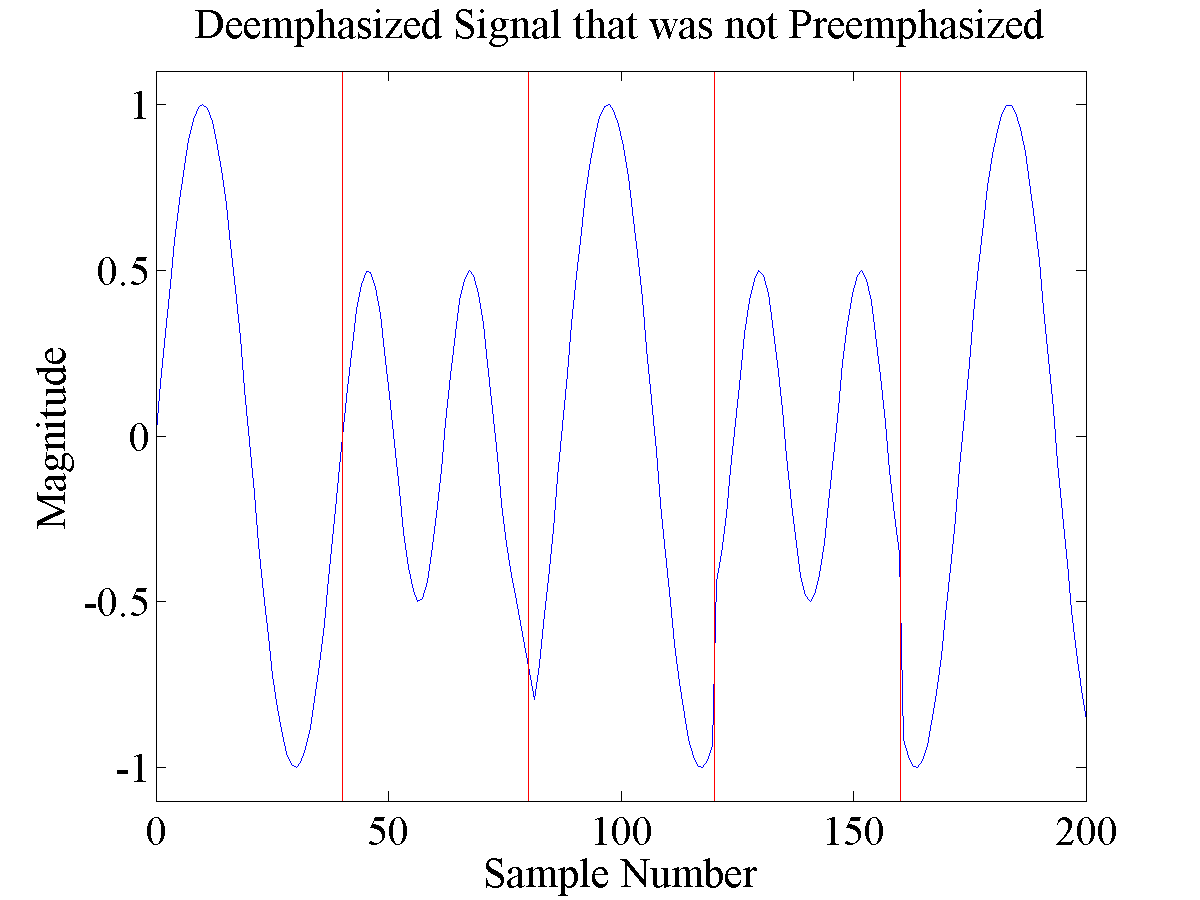
\includegraphics[width=0.75\linewidth]{images/DeemphasizedSignalthatwasnotPreemphasized.png} 
	\caption{An example signal that was not preemphasized, but was deemphasized.}
   \label{emphasisExample}
\end{figure}
